\begin{frame}
	\frametitle{Molten Salt Reactors}
		\begin{itemize}
			\item A class of advanced nuclear reactor concepts that contain
			nuclear fuel dissolved and circulating in a molten salt coolant
			loop
			\item May also include designs with solid fuel and molten salt
			coolant
			\item Can potentially run for extended periods with minimal shutdown
			time due to online fuel reprocessing capabilities
		\end{itemize}
		\begin{figure}
			\centering
			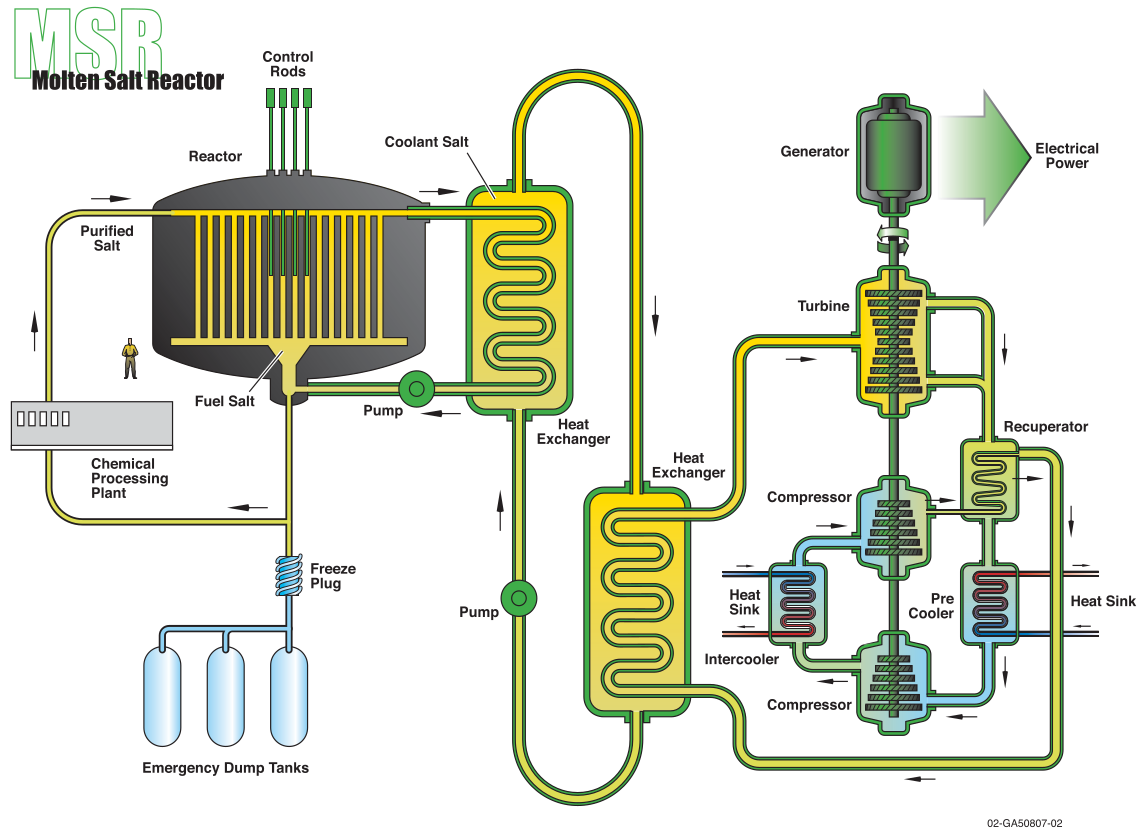
\includegraphics[width=.5\textwidth]{./images/msr}
			\caption{Schematic diagram of a general \gls{MSR} concept.}
			\label{fig:msr}
		\end{figure}
\end{frame}

\begin{frame}
	\frametitle{Molten Salt Reactors}
		\textbf{Characteristics and challenges}
		\begin{itemize}
			\item Strong coupling between neutronics and thermal-hydraulics
			\begin{itemize}
				\item Strong Doppler and density feedback in the fuel salt
				\item Relatively more prompt response expected compared to
				existing LWRs
			\end{itemize}
			\item Movement and decay of \gls{DNP} in the molten
			salt loop
			\begin{itemize}
				\item Conventional safety analysis codes do not account for the
				delayed neutron precursor movement
			\end{itemize}
			\item Constantly evolving fuel composition across the lifetime of an
			\gls{MSR}
			\begin{itemize}
				\item Reactor safety parameters and transient response may be
				different for \gls{BOL} vs \gls{EOL} fuel compositions
			\end{itemize}
		\end{itemize}
\end{frame}
